\documentclass[11pt]{article}

\usepackage[margin=1in]{geometry}
\usepackage[T1]{fontenc}
\usepackage{lmodern}
\usepackage{parskip}
\usepackage{booktabs}
\usepackage{longtable}
\usepackage{array}
\usepackage{xcolor}
\usepackage{listings}
\usepackage{hyperref}
\usepackage{enumitem}
\usepackage{titlesec}
\usepackage{graphicx}

\hypersetup{
    colorlinks=true,
    linkcolor=blue!50!black,
    urlcolor=blue!50!black,
}

\titleformat{\section}{\Large\bfseries}{\thesection}{0.6em}{}
\titleformat{\subsection}{\large\bfseries}{\thesubsection}{0.6em}{}

\lstdefinestyle{codestyle}{
    basicstyle=\ttfamily\small,
    backgroundcolor=\color{gray!8},
    frame=single,
    breaklines=true,
    columns=fullflexible,
    showstringspaces=false,
    xleftmargin=2pt,
    xrightmargin=2pt,
}
\lstset{style=codestyle}

\newcolumntype{L}[1]{>{\raggedright\arraybackslash}p{#1}}

\setlist[itemize]{leftmargin=1.5em, labelsep=0.5em, itemsep=0.3em, topsep=0.3em, rightmargin=0pt, parsep=0pt}
\setlist[enumerate]{leftmargin=1.5em, labelsep=0.5em, itemsep=0.3em, topsep=0.3em, rightmargin=0pt, parsep=0pt}

% Breakable inline code: same look as \texttt (plain black monospace, no
% hyperlink), but allowed to wrap at /, :, _, - like a URL would.
\newcommand{\brk}[1]{\begingroup\urlstyle{tt}\begin{NoHyper}\url{#1}\end{NoHyper}\endgroup}

\title{\textbf{Mini Payment Router Simulator}\\[0.5em]}

\begin{document}

\maketitle

\tableofcontents

\clearpage
% ===========================================================================
\section{App Architecture (Frontend--Backend Interaction)}
% ===========================================================================

The system is five containers wired together by Docker Compose: a React frontend, the
main \texttt{payment-router} backend, two dummy Digital Financial Service Providers
(\texttt{dfsp-a}, \texttt{dfsp-b}), and a PostgreSQL database.

\begin{figure}[h]
\centering
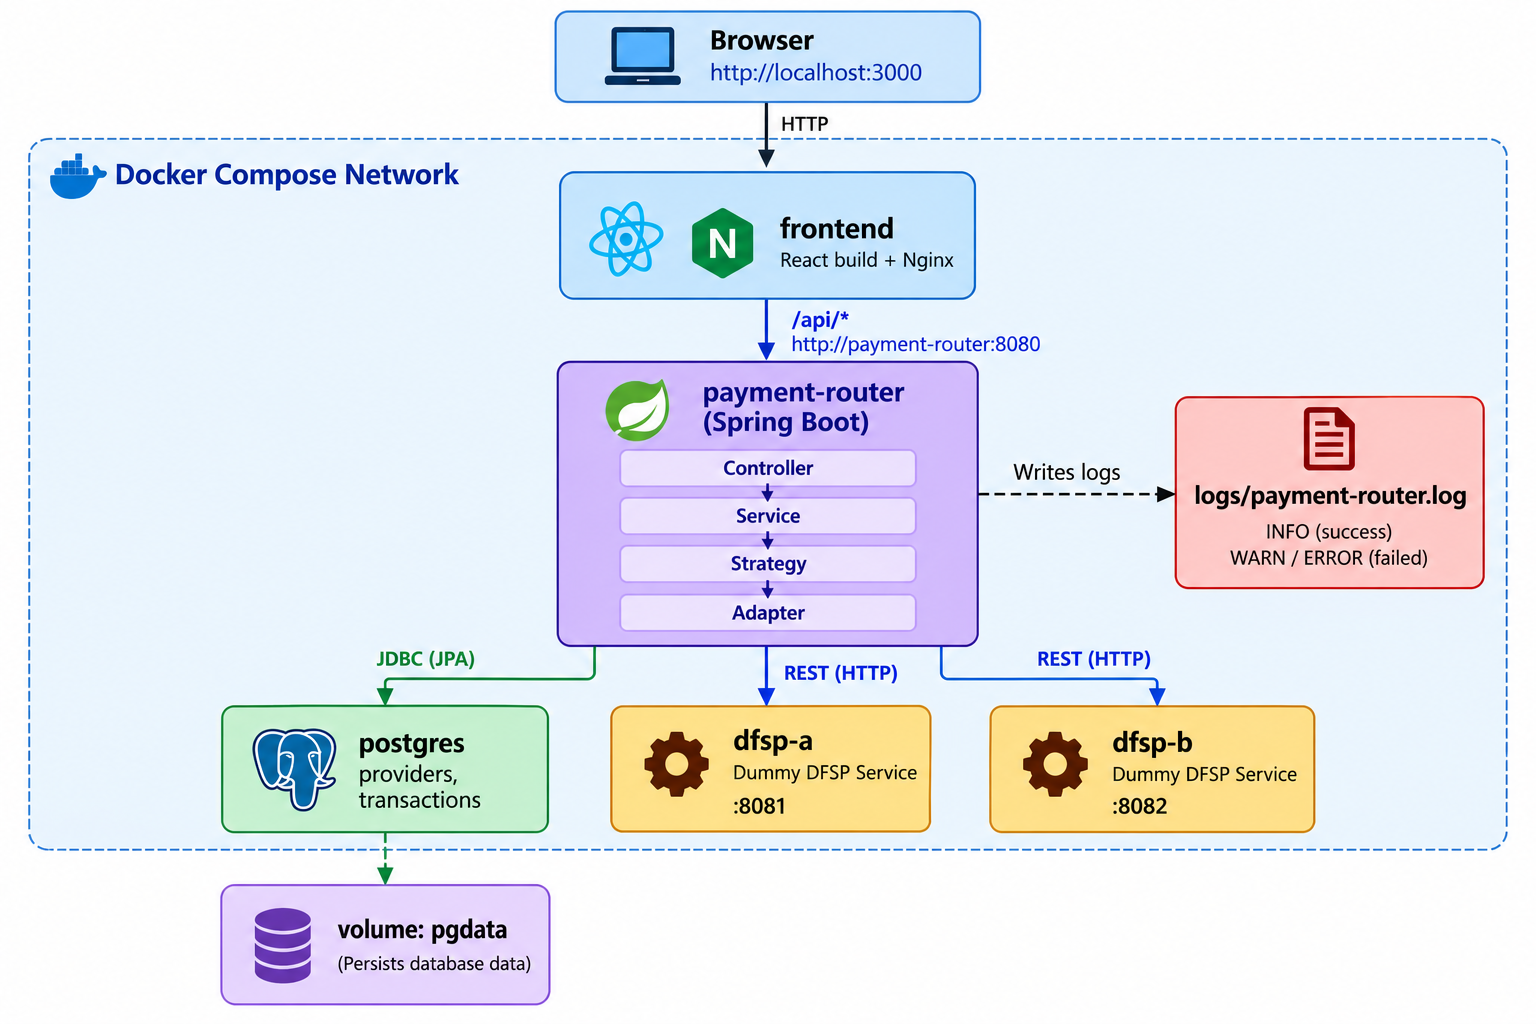
\includegraphics[width=0.95\textwidth]{../architecture-diagram.png}
\caption{Browser to frontend (React + Nginx), to payment-router (Controller
$\rightarrow$ Service $\rightarrow$ Strategy $\rightarrow$ Adapter), to postgres,
dfsp-a and dfsp-b, all inside one Docker Compose network.}
\end{figure}

\subsection*{How the frontend talks to the backend}
\begin{itemize}
\item The browser talks \textbf{only} to \texttt{frontend}. In Docker, \textbf{Nginx}
serves the built React static files and reverse-proxies every \texttt{/api/*} request
to \texttt{payment-router:8080}. In local development, the \textbf{Vite dev server}
proxies \texttt{/api} to \texttt{http://localhost:8080} the same way. Either way, the
browser sees a single origin, so CORS is never involved in the normal path.
\item \textbf{Only \texttt{payment-router} talks to \texttt{postgres}, \texttt{dfsp-a}
and \texttt{dfsp-b}.} The two DFSPs never talk to each other or to the database ---
every cross-service call goes through the router.
\item Containers reach each other by Docker Compose \textbf{service name}
(\texttt{postgres:5432}, \texttt{http://dfsp-a:8081}), never by \texttt{localhost}.
\item A proxy must forward the browser's original \texttt{Host} header (Nginx:
\texttt{proxy\_set\_header Host \$http\_host}). If it did not, Spring would see a
mismatched Origin/Host on a POST and reject it as a cross-origin request.
\end{itemize}

\subsection*{Runtime interaction, step by step}
\begin{enumerate}
\item The frontend loads on \texttt{http://localhost:3000} and calls \texttt{GET
/api/providers} to populate the source/destination dropdowns --- nothing is
hard-coded in the UI.
\item The user picks a source, a destination and an amount, then clicks
\textbf{Get quote}. The frontend calls \texttt{POST /api/quotes}. Nothing is sent to
a DFSP and nothing is saved; it is a pure calculation.
\item The user clicks \textbf{Confirm transfer}. The frontend calls \texttt{POST
/api/transfers} with the same three fields. This time the router actually calls the
destination DFSP over HTTP, waits for its answer, and saves exactly one row in
PostgreSQL --- \texttt{SUCCESS} or \texttt{FAILED}, either way.
\item The frontend renders the result card returned by that call: status badge,
transaction ID, the DFSP's own message, and the pricing snapshot. The frontend holds
no business logic of its own --- every number shown came from the backend response.
\end{enumerate}

\subsection*{Layering inside \texttt{payment-router}}
\begin{lstlisting}
Controller -> Service -> DfspStrategy -> DfspClient (adapter) -> DFSP over HTTP
                |
                +------> Repository -> PostgreSQL
\end{lstlisting}

\clearpage
% ===========================================================================
\section{Key Code Components and Their Purpose}
% ===========================================================================

\subsection{Packages inside \texttt{payment-router}}

\begin{longtable}{L{0.20\textwidth} L{0.70\textwidth}}
\toprule
\textbf{Package} & \textbf{Responsibility} \\
\midrule
\endhead
\texttt{controller} & HTTP endpoints; triggers \texttt{@Valid}; delegates to
services \\
\texttt{service} & Business validation, quote calculation, transfer
orchestration; picks the strategy matching the destination provider's code \\
\texttt{strategy} & One strategy per DFSP (pricing + which adapter to call) \\
\texttt{client} & Adapters translating to and from each DFSP's own API \\
\texttt{entity}, \texttt{repository} & JPA entities and Spring Data repositories \\
\texttt{exception} & Custom exceptions and the global error handler \\
\texttt{config} & HTTP client timeouts, CORS, provider seed data \\
\bottomrule
\end{longtable}

\subsection{The five services and what each one owns}
\begin{itemize}
\item \textbf{Frontend} --- a form for source/destination/amount; shows the quote and
the transfer result; contains no business logic.
\item \textbf{Payment Router} --- validates requests, calculates quotes, routes
transfers via the right strategy/adapter, saves every attempt, and logs events. This
is the only "smart" component in the system.
\item \textbf{DFSP-A} --- dummy provider, its own API format, rejects transfers above
50{,}000.00 taka.
\item \textbf{DFSP-B} --- dummy provider, a deliberately different API format (paisa,
different field names), rejects transfers above 25{,}000.00 taka.
\item \textbf{PostgreSQL} --- stores providers and transactions only; reachable only
by \texttt{payment-router}.
\end{itemize}

\subsection{Strategy Pattern --- isolates DFSP-specific behaviour}

The interface \texttt{DfspStrategy} declares three operations: \texttt{getProviderCode()},
\texttt{calculateQuote(amount, destinationProvider)} and
\texttt{executeTransfer(request, destinationProvider)}. \texttt{DfspAStrategy} and
\texttt{DfspBStrategy} each implement it. \texttt{calculateQuote} has one common
default implementation on the interface itself (fee = amount $\times$
fee\_percentage / 100, rounded \texttt{HALF\_UP}; total = amount + fee), since both
DFSPs currently price the same way; a DFSP whose pricing ever differs would simply
override that one method.

Each strategy's \texttt{executeTransfer} routes to its own \texttt{DfspClient}
adapter (\texttt{DfspAStrategy} $\rightarrow$ \texttt{DfspAAdapter},
\texttt{DfspBStrategy} $\rightarrow$ \texttt{DfspBAdapter}). \texttt{TransferService}
and \texttt{QuoteService} never write \texttt{if\allowbreak{} (code.equals(\allowbreak{}"DFSP\_A"))\allowbreak{} ...}; they
ask "give me the strategy for this provider code" (a
\texttt{stream().filter()} lookup over the injected list of strategies) and call it.
Adding a third DFSP means adding one new strategy class, not editing existing logic.

\subsection{Adapter Pattern --- hides DFSP API differences}

\texttt{DfspTransferRequest} and \texttt{DfspTransferResult} are the router's common,
DFSP-neutral models. The interface \texttt{DfspClient} declares a single method,
\texttt{transfer(baseUrl, DfspTransferRequest)}, implemented by \texttt{DfspAAdapter}
and \texttt{DfspBAdapter}.

\begin{longtable}{L{0.22\textwidth} L{0.34\textwidth} L{0.34\textwidth}}
\toprule
\textbf{Adapter} & \textbf{Translates request to} & \textbf{Translates response
from} \\
\midrule
\endhead
\texttt{DfspAAdapter} & Decimal taka, DFSP-A's own field names &
\texttt{"SUCCESS"}/\texttt{"FAILED"} $\rightarrow$ common \texttt{SUCCESS}/\texttt{FAILED} \\
\texttt{DfspBAdapter} & Integer paisa, DFSP-B's own field names &
\texttt{"ACCEPTED"}/\texttt{"REJECTED"} $\rightarrow$ common \texttt{SUCCESS}/\texttt{FAILED} \\
\bottomrule
\end{longtable}

Each adapter sends its DFSP-specific JSON to the provider's \texttt{base\_url} (read
from the \texttt{providers} table) and converts the reply back into the common model.
Network errors (DFSP down, timeout) become a \texttt{DfspCommunicationException},
which the transfer service turns into a \texttt{FAILED} transaction rather than an
HTTP error. Timeouts are configurable: \texttt{dfsp.client.connect-timeout=3s},
\texttt{dfsp.client.read-timeout=5s}.

\clearpage
% ===========================================================================
\section{How the API Works Internally}
% ===========================================================================

Every request follows the same internal path before any business logic runs:
\texttt{Controller} receives the HTTP call, Spring's \texttt{@Valid} annotation
triggers field-level validation on the request DTO first, and only a structurally
valid request reaches \texttt{PaymentRequestValidator} for business-level checks
(does the provider exist, is it active). Only after both checks pass does the
\texttt{Service} layer pick a \texttt{DfspStrategy} and, for a transfer, call the
matching \texttt{DfspClient} adapter and save the outcome.

\subsection{Endpoints}

\begin{longtable}{L{0.12\textwidth} L{0.28\textwidth} L{0.50\textwidth}}
\toprule
\textbf{Method} & \textbf{Path} & \textbf{Purpose} \\
\midrule
\endhead
POST & \texttt{/api/quotes} & Calculate a quote (nothing is saved) \\
POST & \texttt{/api/transfers} & Execute a transfer (a transaction is saved) \\
GET & \texttt{/api/providers} & List providers (UI dropdowns) \\
GET & \texttt{/api/status} & Service status (used by the Docker healthcheck) \\
\bottomrule
\end{longtable}

\subsection{Quote}
\texttt{POST /api/quotes}
\begin{lstlisting}
{ "sourceProviderCode": "DFSP_A", "destinationProviderCode": "DFSP_B", "amount": 1000.00 }
\end{lstlisting}
\texttt{200 OK}
\begin{lstlisting}
{
  "sourceProviderCode": "DFSP_A",
  "destinationProviderCode": "DFSP_B",
  "amount": 1000.00,
  "feePercentage": 1.50,
  "feeAmount": 15.00,
  "totalAmount": 1015.00
}
\end{lstlisting}

\subsection{Transfer}
\texttt{POST /api/transfers} has the same request body as a quote.

\texttt{201 Created}. A transaction row is created for SUCCESS and for FAILED; the
business outcome is in \texttt{status}.
\begin{lstlisting}
{
  "transactionId": "3f6e2c1a-8b0d-4c5e-9a4f-1d2b3c4d5e6f",
  "sourceProviderCode": "DFSP_A",
  "destinationProviderCode": "DFSP_B",
  "amount": 1000.00,
  "feePercentage": 1.50,
  "feeAmount": 15.00,
  "totalAmount": 1015.00,
  "status": "SUCCESS",
  "message": "ACCEPTED (ref B-PAY-000123)",
  "createdAt": "2026-09-14T10:01:12Z"
}
\end{lstlisting}

\subsection{Error response (all endpoints)}
\begin{lstlisting}
{
  "timestamp": "2026-09-14T10:01:12Z",
  "status": 400,
  "error": "Bad Request",
  "message": "Provider not found: DFSP_X",
  "fieldErrors": {}
}
\end{lstlisting}

\begin{longtable}{L{0.12\textwidth} L{0.78\textwidth}}
\toprule
\textbf{HTTP} & \textbf{When} \\
\midrule
\endhead
400 & Field validation failed, malformed JSON, provider not found or inactive \\
404 & No endpoint for the URL \\
405 & HTTP method not supported by the endpoint \\
415 & Body not sent as \texttt{application/json} \\
500 & Unexpected server error (details only in the log) \\
\bottomrule
\end{longtable}

All of these are produced by \texttt{GlobalExceptionHandler} with the same JSON
shape. A DFSP timeout gets its own FAILED message: ``Destination DFSP did not
respond in time''. DFSP rejection or DFSP unavailability is \textbf{not} an HTTP
error for the client --- it is saved and returned as a \texttt{FAILED} transaction.

\subsection{Validation}

\begin{longtable}{L{0.38\textwidth} L{0.22\textwidth} L{0.30\textwidth}}
\toprule
\textbf{Rule} & \textbf{Where} & \textbf{Mechanism} \\
\midrule
\endhead
Amount is required and greater than zero & Request DTO & \texttt{@NotNull},
\texttt{@Positive} + \texttt{@Valid} \\
At most 9 integer digits, 2 decimal places & Request DTO &
\texttt{@Digits(integer = 9, fraction = 2)} \\
Source provider is required & Request DTO & \texttt{@NotBlank} \\
Destination provider is required & Request DTO & \texttt{@NotBlank} \\
Provider exists and is ACTIVE & \texttt{PaymentRequest\allowbreak{}Validator} & DB lookup
$\rightarrow$ 400 \\
\bottomrule
\end{longtable}

Source and destination are \textbf{allowed to be the same provider}. A DFSP sending
a payment to itself (e.g.\ \texttt{DFSP\_A} $\rightarrow$ \texttt{DFSP\_A}) is
validated, priced and routed exactly like any other transfer, using that provider's
own strategy and adapter.

\texttt{GlobalExceptionHandler} (\texttt{@RestControllerAdvice}) converts
\texttt{MethodArgumentNotValidException} (field errors) and
\texttt{InvalidPaymentRequestException} (business rules) into the error JSON above.
Quote and transfer share the same business checks through
\texttt{PaymentRequestValidator}. The 9-digit limit keeps \texttt{amount + fee}
inside the \texttt{NUMERIC(12,2)} columns, so a very large amount is rejected with
400 instead of failing when the transaction is saved.

\clearpage
% ===========================================================================
\section{Docker Setup Explanation}
% ===========================================================================

\begin{longtable}{L{0.16\textwidth} L{0.34\textwidth} L{0.18\textwidth} L{0.20\textwidth}}
\toprule
\textbf{Service} & \textbf{Image / build} & \textbf{Port (host:container)} &
\textbf{Depends on} \\
\midrule
\endhead
\texttt{frontend} & \texttt{node:22-alpine} build $\rightarrow$
\texttt{nginx:1.27-alpine} & \brk{${FRONTEND_PORT:-3000}:80} &
payment-router (healthy) \\
\texttt{payment-router} & \texttt{maven:3.9-eclipse-temurin-21} build
$\rightarrow$ \texttt{eclipse-temurin:21-jre-alpine} & \texttt{8080:8080} &
postgres (healthy), dfsp-a, dfsp-b \\
\texttt{dfsp-a} & Maven build $\rightarrow$ \texttt{eclipse-temurin:21-jre-alpine}
& \texttt{8081:8081} & -- \\
\texttt{dfsp-b} & Maven build $\rightarrow$ \texttt{eclipse-temurin:21-jre-alpine}
& \texttt{8082:8082} & -- \\
\texttt{postgres} & \texttt{postgres:16-alpine} & not published & -- \\
\bottomrule
\end{longtable}

\begin{itemize}
\item \textbf{Multi-stage Dockerfiles.} Build tools (Maven, Node) stay in the build
stage; the final image only contains what is needed to run.
\item \textbf{Healthcheck on postgres} (\texttt{pg\_isready}).
\texttt{payment-router} waits for \texttt{condition: service\_healthy}, so it does
not start before the DB accepts connections.
\item \textbf{Healthcheck on payment-router} (\texttt{wget} \brk{http://localhost:8080/api/status}
inside its own container). \texttt{frontend}
waits until the router is healthy.
\item \textbf{Tests are not run inside the image build} (\texttt{-DskipTests}),
because the router's tests need PostgreSQL. Run them with \texttt{./mvnw test}
before building.
\item \textbf{Nginx} (\texttt{frontend/nginx.conf}) serves the React build and
proxies \texttt{/api/} to \brk{http://payment-router:8080} with \texttt{Host
\$http\_host}.
\item \textbf{\texttt{.env.example}} lists the optional overrides
(\texttt{POSTGRES\_DB}, \texttt{POSTGRES\_USER}, \texttt{POSTGRES\_PASSWORD},
\texttt{FRONTEND\_PORT}). Every value has a default in \texttt{docker-compose.yml}.
\item \textbf{Named volume \texttt{pgdata}} keeps database data across restarts.
\item \textbf{Bind mount \texttt{./logs:/app/logs}} makes the log file visible on
the host.
\item \textbf{Environment variables} configure the DB connection
(\brk{SPRING_DATASOURCE_URL=jdbc:postgresql://postgres:5432/payment_router},
username, password).
\item DFSP addresses come from \texttt{providers.base\_url}. In Docker they are
seeded as service names through \brk{DFSP_A_BASE_URL=http://dfsp-a:8081} and
\brk{DFSP_B_BASE_URL=http://dfsp-b:8082}.
\item Start everything with \texttt{docker compose up --build}, then open
\texttt{http://localhost:3000}.
\end{itemize}

\clearpage
% ===========================================================================
\section{Additional Notes: Design Decisions and Testing}
% ===========================================================================

\subsection{Notable design decisions}

\begin{longtable}{L{0.42\textwidth} L{0.50\textwidth}}
\toprule
\textbf{Decision} & \textbf{Why} \\
\midrule
\endhead
Fee priced from the \textbf{destination} provider, not the source &
Whoever receives and processes a payment sets its price --- mirrors how real
inter-DFSP settlement works \\
Pricing snapshot stored on every transaction &
A fee changed tomorrow must never rewrite what a transfer cost yesterday \\
Every valid attempt is saved, success or failure &
A rejected, timed-out or unreachable transfer is still a business event, not an
error to discard \\
Database write happens \emph{after} the DFSP call, never wrapping it &
A slow or hanging DFSP must never hold a database connection open \\
Two DFSP APIs made deliberately incompatible &
Gives the Adapter Pattern a genuine reason to exist --- taka vs paisa,
\texttt{SUCCESS}/\texttt{FAILED} vs \texttt{ACCEPTED}/\texttt{REJECTED} \\
Strategy selection is a \texttt{stream().filter()}, no factory class &
Only two DFSPs; a dedicated lookup class is pure overhead. Adding DFSP-C means
one new strategy + adapter bean, nothing else changes \\
Source and destination may be the same provider &
A DFSP paying itself is still a valid transfer; there's no reason to
special-case it \\
\texttt{spring.jpa.open-in-view=false} &
Forces every database read to finish inside the service layer; a stray
lazy-load reached from a controller fails loudly instead of silently \\
Nginx forwards the browser's original \texttt{Host} header &
Otherwise Spring sees a mismatched Origin/Host and rejects the POST as
cross-origin \\
\texttt{BigDecimal} / \texttt{NUMERIC} for every amount &
Binary floating point cannot represent \texttt{15.00} exactly, and a fee is
not an approximation \\
No quotes table &
A quote is a calculation, not a record --- nothing to persist \\
No authentication &
Out of scope for this assessment \\
\bottomrule
\end{longtable}

\subsection{Tests}

\begin{lstlisting}
cd backend/payment-router && ./mvnw test   # 56 tests
cd backend/dfsp-a         && ./mvnw test   # 5 tests
cd backend/dfsp-b         && ./mvnw test   # 5 tests
\end{lstlisting}

The router's tests run against a \textbf{real PostgreSQL} on port 5433, not an
in-memory database --- \texttt{NUMERIC} precision and constraint behaviour need to be
exercised as they actually behave. The adapter tests (\texttt{DfspAAdapterTest},
\texttt{DfspBAdapterTest}) start a tiny real local HTTP server standing in for the
DFSP (the JDK's own \texttt{HttpServer}, no test framework involved), so the JSON the
adapter actually sends and the response it actually parses are both exercised over a
real socket.

\begin{lstlisting}
docker compose up --build -d
bash scripts/smoke-test.sh   # 21 checks against the real Compose stack, through Nginx
\end{lstlisting}

The smoke test is the only place the full request $\rightarrow$ validation
$\rightarrow$ strategy $\rightarrow$ adapter $\rightarrow$ DFSP $\rightarrow$
database $\rightarrow$ response chain is exercised end to end, against the real
stack --- deliberately the one place this project uses a real HTTP client instead of
an in-process HTTP-layer testing tool. There is no frontend test suite.

\end{document}
